\worksheet{FIFA Octopus Oracle}

\textbf{Paul the Octopus's Predictions}

Let's make FIFA predations by guessing,

\begin{enumerate}
	\item Flip a coin 14 times.
	\item Keep track of the number of heads and tails in the grid below.
	\item You match Paul's unlikeliness by getting heads 2 or 12 times.
	\item You beat Paul's unlikeliness by getting heads 0, 1, 13, or 14 times.
	
		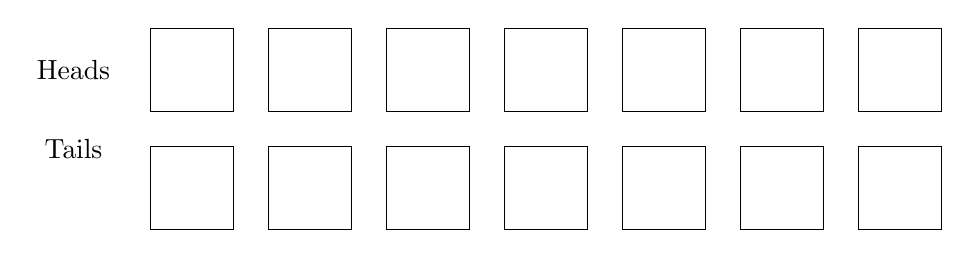
\begin{tikzpicture}
	\node at (0,0) {Heads};
		 \foreach \x in {1,...,7}{
       \node [inner sep=15pt, draw] at  (1.5*\x,0)  {};
       }
	\node at (0, -1) {Tails};
		 \foreach \x in {1,...,7}{
       \node [inner sep=15pt, draw] at  (1.5*\x,-1.5)  {};
       }
	\end{tikzpicture}
	
\noindent\rule[0.5ex]{\linewidth}{1pt}
	
		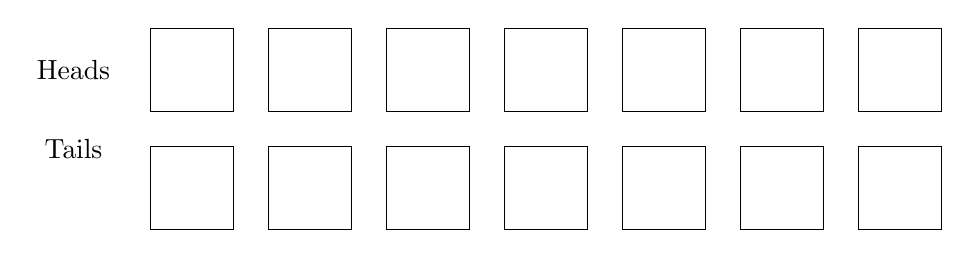
\begin{tikzpicture}
	\node at (0,0) {Heads};
		 \foreach \x in {1,...,7}{
       \node [inner sep=15pt, draw] at  (1.5*\x,0)  {};
       }
	\node at (0, -1) {Tails};
		 \foreach \x in {1,...,7}{
       \node [inner sep=15pt, draw] at  (1.5*\x,-1.5)  {};
       }
	\end{tikzpicture}
	
	Just as before, it is quicker to use the Bernoulli formula to calculate these probabilities exactly:
	\[ \text{The probability of \(r\) successes out of \(n\) attempts where the probability of each success is \(p\) } = C(n,r)\times p^r \times p^{n-r}\] 
	\item Calculate the probability that you match Paul's unlikeliness using the Bernoulli formula.
	\vfill
		\item Calculate the probability that you beat Paul's unlikeliness using the Bernoulli formula.
	\vfill
	
	\item In statistics, as a rule of thumb, we say that something is rare if the probability that it happens is less than 5\%. Which of the two outcomes could we call rare? Do you agree? \vfill
\end{enumerate}